\tikzstyle{inner} = [circle, minimum size = 0.4cm, draw, inner sep = 0.1pt]
\tikzstyle{inner_g} = [inner, fill = green]

    
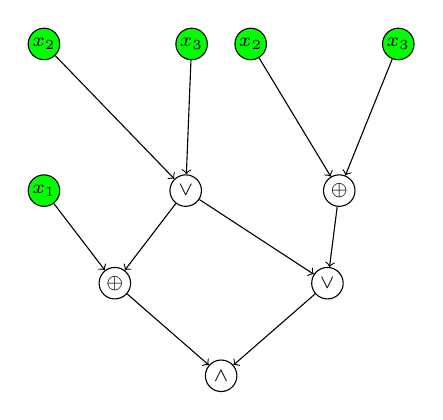
\begin{tikzpicture}[yscale = -0.98, xscale = 1.5]
    \node[inner] (a) at (0, 0) {\scriptsize $\land$};
    \node[inner] (b) at (-0.9, -1.2) {\scriptsize $\oplus$};
    \node[inner] (c) at (0.9, -1.2) {\scriptsize $\lor$};
    \node[inner_g] (d) at (-1.5, -2.4) {\scriptsize $x_1$};
    \node[inner] (e) at (-0.3, -2.4) {\scriptsize $\lor$};
    \node[inner] (f) at (1, -2.4) {\scriptsize $\oplus$};
    \node[inner_g] (g) at (-1.5, -4.3) {\scriptsize $x_2$};
    \node[inner_g] (h) at (-0.25, -4.3) {\scriptsize $x_3$};
    \node[inner_g] (g2) at (1.5, -4.3) {\scriptsize $x_3$};
    \node[inner_g] (h2) at (0.25, -4.3) {\scriptsize $x_2$};

    \draw[<-] (a) -- (b);
    \draw[<-] (a) -- (c);
    \draw[<-] (b) -- (d);
    \draw[<-] (b) -- (e);
    \draw[<-] (c) -- (e);
    \draw[<-] (c) -- (f);
    \draw[<-] (e) -- (g);
    \draw[<-] (e) -- (h);
    \draw[<-] (f) -- (g2);
    \draw[<-] (f) -- (h2);
\end{tikzpicture}
